\mode*

% Since this a solution template for a generic talk, very little can
% be said about how it should be structured. However, the talk length
% of between 15min and 45min and the theme suggest that you stick to
% the following rules:  

% - Exactly two or three sections (other than the summary).
% - At *most* three subsections per section.
% - Talk about 30s to 2min per frame. So there should be between about
%   15 and 30 frames, all told.


\section{Introduction}

\subsection{What are side-channels?}

\begin{frame}
  \begin{definition}[Side Channel]
    \begin{itemize}
      \item Unintended channel emitting information.
      \item Due to physical implementation flaws and not theoretical weaknesses 
        or forcing attempts.
    \end{itemize}
  \end{definition}
\end{frame}

\begin{frame}
  \begin{itemize}
    \item There are various categories, \eg
      \begin{itemize}
        \item timing attacks,
        \item acoustic attacks,
        \item electromagnetic attacks,
        \item \dots
      \end{itemize}
  \end{itemize}
\end{frame}


\section{Timing attacks}

\subsection{Doing arithmetic}

\begin{frame}
  \begin{example}
    \begin{itemize}
      \item Use the standard algorithms for addition and multiplication (using 
        the binary number system).
      \item Give any number to an algorithm \(A\).
      \item \(A\) will multiply your number by a secret value \(x\).
      \item Can you tell the difference between \(x = 3\) or \(x = 7\)?
    \end{itemize}
  \end{example}
\end{frame}

\begin{frame}
  \begin{itemize}
    \item Assume that we give the number \(25\) as our challenge to \(A\).
    \item Looking at the numbers we have we see that \(3_{10} = 11_2\), 
      \(7_{10} = 111_2\) and \(25_{10} = 11001_2\)

    \item Assume each step in the algorithm takes one time unit.

    \item Then \(11001\times 11\) will take \(17\) time units:
      \begin{itemize}
        \item \(5\) time units for multiplying the last \(1\) in \(11\) with 
          each digit in \(11001\),

        \item another \(5\) time units for the next digit in \(11\),

        \item we have an additional \(1\) time unit for shifting the second 
          result one step,

        \item finally, we get \(6\) time units for adding the numbers.
      \end{itemize}

    \item \(11001\times 111\) will take \(24\) time units:
      \begin{itemize}
        \item \(5\) time units for each digit, hence \(15\) in total,

        \item we have two shifts, thus \(2\) time units more,

        \item finally we have \(7\) time units for adding.
      \end{itemize}
  \end{itemize}
\end{frame}

\begin{frame}
  \begin{remark}
    \begin{itemize}
      \item The first multiplication takes \(17\) time units to perform,
        the second takes \(24\) time units.

      \item This is one example of why \emph{constant-time operations} are 
        desirable.
    \end{itemize}
  \end{remark}

  \pause

  \begin{exercise}
    \begin{itemize}
      \item Can we see the difference between \(x = 2_{10} = 10_2\) and \(x = 
          3_{10} = 11_2\)?
    \end{itemize}
  \end{exercise}
\end{frame}

\subsection{Typing pattern and guessing passwords}

\begin{frame}
  \begin{example}[SSH password guessing]
    \begin{itemize}
      \item \Textcite{song2001timing} showed a timing attack on passwords sent 
        over encrypted SSH sessions.

      \item As each keystroke in the password is sent in a separate package, 
        the attacker can observe the delay between keystrokes.

      \item They found that this gave a factor 50 advantage for guessing the 
        password.
    \end{itemize}
  \end{example}
\end{frame}

\begin{frame}
  \begin{remark}
    \begin{itemize}
      \item Analytics scripts on many websites send key-presses to the server as 
        you type.
      \item That's exactly the same situation.
    \end{itemize}
  \end{remark}
\end{frame}

\subsection{Summary}

\begin{frame}
  \begin{itemize}
    \item We can measure the time for different operations.
    \item Depending on the operations and times they take, we can figure out 
      something about the operands.
  \end{itemize}
\end{frame}


\section{Emission attacks}

\subsection{Emissions from electronic systems}

\begin{frame}
  \begin{itemize}
    \item Electronic systems emit signals just by running.
    \item Remember induction and similar properties from physics class.
    \item \Eg electromagnetic emissions or acoustic emissions from vibrations.
  \end{itemize}
\end{frame}

\subsection{Exploiting acoustic emissions}

\begin{frame}
  \begin{itemize}
    \item Some authors\footfullcite{AcousticKeyExtraction} showed an attack to 
      extract a 4096-bit RSA private key from a laptop PC (GnuPG implementation 
      of RSA).

    \item Computers emit high-pitched noise during operation due to vibrations 
      in some of their electronic components.

    \item This was used to derive the key used for decryption of some chosen 
      ciphertexts within an hour!

    \item Their results show that this attack can be accomplished by placing 
      a mobile phone (microphone) next to the target laptop.
  \end{itemize}
\end{frame}

\begin{frame}
  \begin{figure}
    \includegraphics[height=0.4\textheight]{acoustic-setup.jpg}
  \end{figure}
  \begin{figure}
    \includegraphics[height=0.4\textheight]{acoustic-mobile.jpg}
  \end{figure}
\end{frame}

\begin{frame}
  \begin{figure}
    \includegraphics[height=0.45\textheight]{acoustic-spectrum.jpg}
  \end{figure}
  \begin{itemize}
    \item The acoustic signals are picked up from components in the power 
      supply.

    \item Individual CPU operations are too fast for a microphone to pick up.

    \item But long operations such as modular exponentiation (as in RSA) can 
      create a characteristic acoustic spectral signature which can be detected 
      using a microphone.
  \end{itemize}
\end{frame}

\begin{frame}
  \begin{figure}
    \includegraphics[width=\textwidth]{acoustic-bits.jpg}
  \end{figure}
\end{frame}

\subsection{Exploiting voltage}

\begin{frame}
  \begin{itemize}
    \item The same authors\footfullcite{VoltageKeyExtraction} did the same thing 
      again, but with variations in the ground--electric potential.
  \end{itemize}
\end{frame}

\begin{frame}
  \begin{figure}
    \includegraphics[width=\textwidth]{physical-setup.png}
  \end{figure}
\end{frame}

\begin{frame}
  \begin{figure}
    \includegraphics[width=\textwidth]{physical-ethernet.png}
  \end{figure}
\end{frame}

\begin{frame}
  \begin{figure}
    \includegraphics[width=\textwidth]{physical-human.png}
  \end{figure}
\end{frame}

\begin{frame}
  \begin{figure}
    \includegraphics[height=0.9\textheight]{physical-spectrum.png}
  \end{figure}
\end{frame}

\subsection{Exploiting electromagnetic emissions}

\begin{frame}
  \begin{itemize}
    \item And again\footfullcite{ElectromagneticKeyExtraction}, but with 
      electromagnetic emissions.
  \end{itemize}
\end{frame}

\begin{frame}
  \begin{figure}
    \includegraphics[height=\textheight]{em-spectrum.png}
  \end{figure}
\end{frame}

\begin{frame}
  \begin{figure}
    \includegraphics[width=\textwidth]{em-pita.png}
  \end{figure}
\end{frame}

\begin{frame}
  \begin{figure}
    \includegraphics[width=\textwidth]{em-pita-detailed.png}
  \end{figure}
\end{frame}

\begin{frame}
  \begin{remark}
    \begin{itemize}
      \item There are also other parts emitting electromagnetic signals.
      \item \Eg screens~\cite{FlatPanelEmissions}.
    \end{itemize}
  \end{remark}
\end{frame}

\begin{frame}
  \begin{figure}
    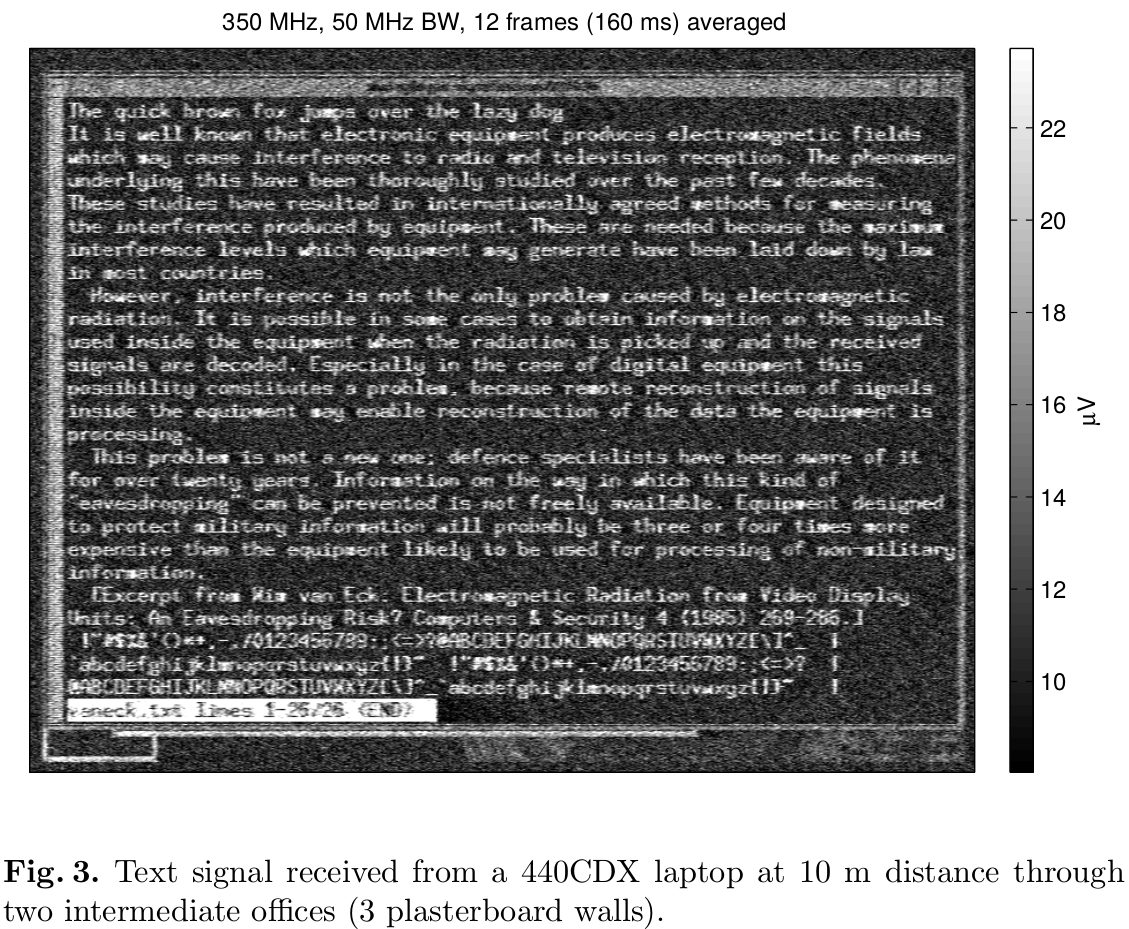
\includegraphics[height=0.9\textheight]{em-laptop.png}
  \end{figure}
\end{frame}

\section{Summary}

\begin{frame}
  \begin{itemize}
    \item We can measure something during the operations.
    \item From these measurements we can infer things about operands \etc.
  \end{itemize}
\end{frame}



%%%%%%%%%%%%%%%%%%%%%%

\begin{frame}[allowframebreaks]
  \small
  \printbibliography{}
\end{frame}

